\documentclass{standalone}
\usepackage{tikz}
% create a new adjust box
\usepackage{tikzscale}
\usepackage{lscape}
\usepackage{tikz}
% use to adjust the positionS
\usetikzlibrary{positioning}
\usetikzlibrary{calc}
\tikzset{abs1/.style={xshift=3cm,yshift=2cm}}
\usetikzlibrary{shapes.geometric,arrows}
\tikzstyle{arrow}=
[thick,->,>=stealth]


\begin{document}
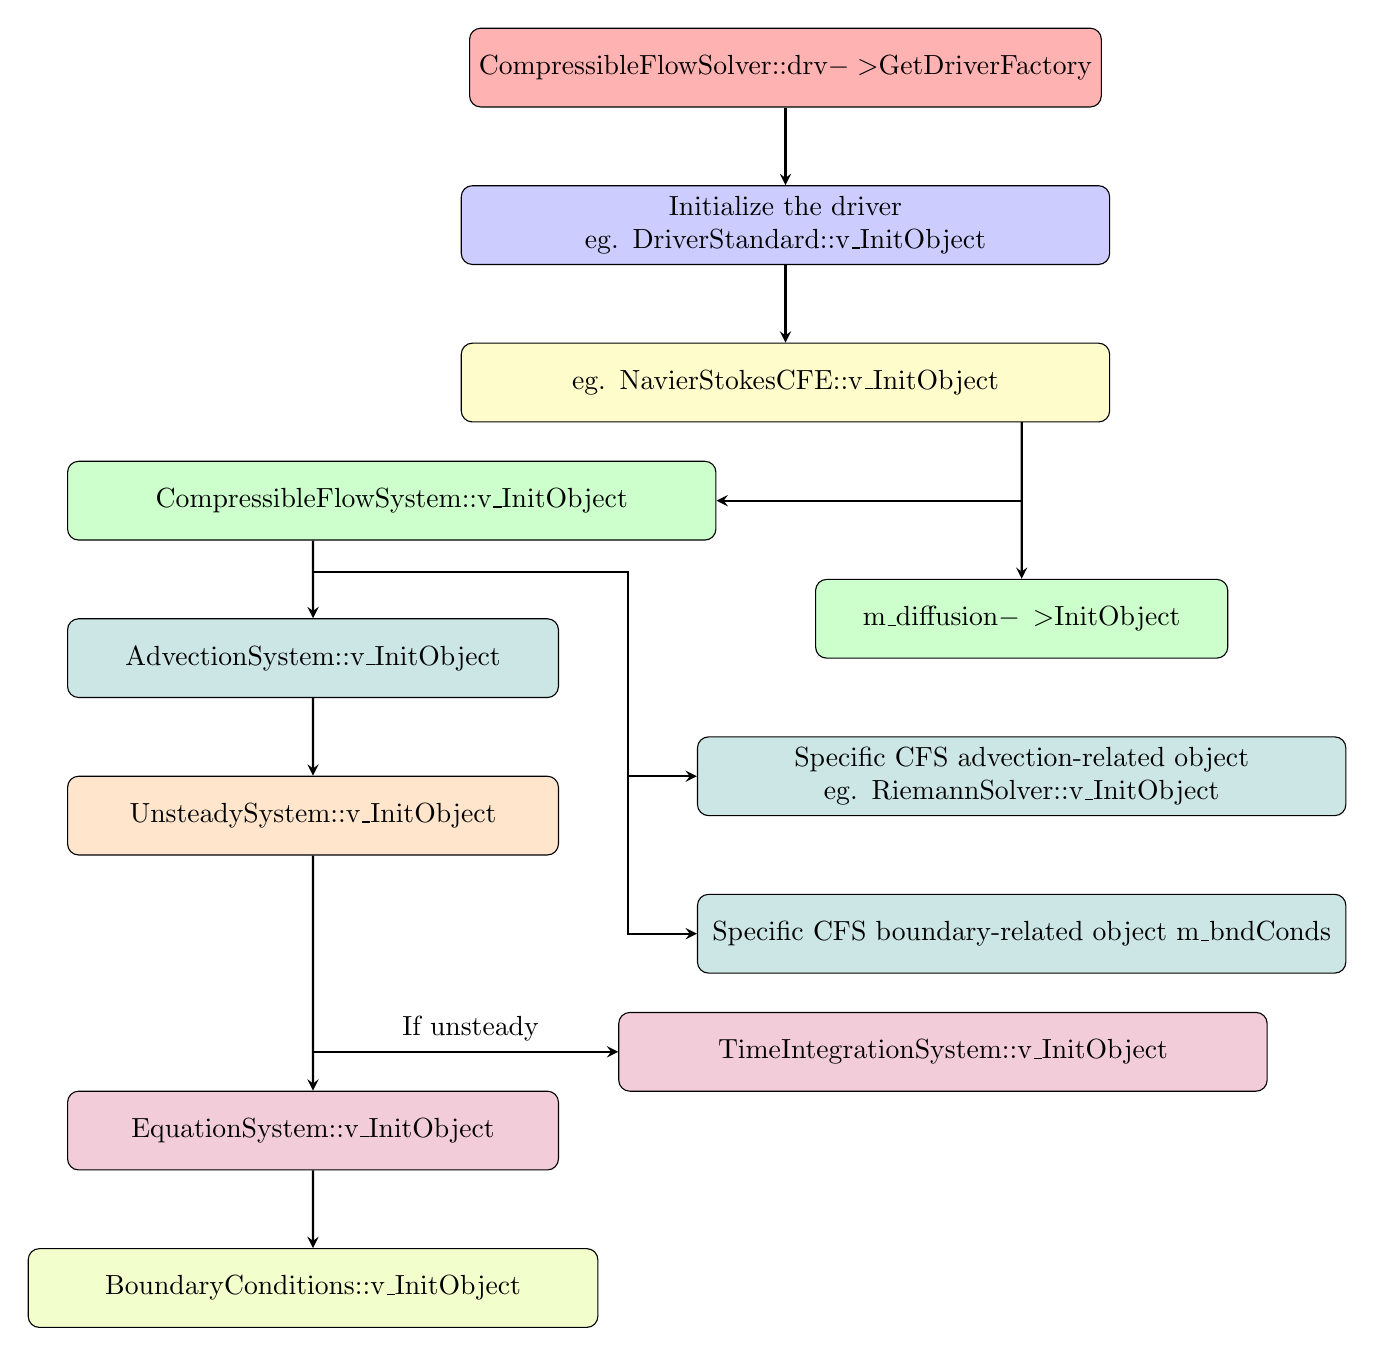
\begin{tikzpicture}[scale=0.2,node distance=2cm]
\node (A)
[rectangle,
rounded corners,
minimum width=3cm,
minimum height=1cm,
text centered,
draw=black,
fill=red!30]
{CompressibleFlowSolver::drv$->$GetDriverFactory};
\node (B)
[rectangle,
rounded corners,
minimum width=8cm,
minimum height=1cm,
text width=8cm,
text centered,
draw=black,
fill=blue!20,
below of=A,
xshift=0cm,
yshift=0cm]
{Initialize the driver\\eg. DriverStandard::v$\_$InitObject};
\draw[arrow](A)--(B);
\node (C)
[rectangle,
rounded corners,
minimum width=8cm,
minimum height=1cm,
text width=8cm,
text centered,
draw=black,
fill=yellow!20,
below of=B,
xshift=0cm,
yshift=0cm]
{eg. NavierStokesCFE::v$\_$InitObject};
\draw[arrow](B)--(C);
\node (D_1)
[rectangle,
rounded corners,
minimum width=8cm,
minimum height=1cm,
text width=8cm,
text centered,
draw=black,
fill=green!20,
below of=C,
xshift=-5cm,
yshift=0.5cm]
{CompressibleFlowSystem::v$\_$InitObject};
\draw[arrow]($(C.south)+(15cm,0)$)|-(D_1);
\node (D_2)
[rectangle,
rounded corners,
minimum width=5cm,
minimum height=1cm,
text width=5cm,
text centered,
draw=black,
fill=green!20,
below of=C,
xshift=3cm,
yshift=-1cm]
{m$\_$diffusion$->$InitObject};
\draw[arrow]($(C.south)+(15cm,0)$)--(D_2);
\node (E_1)
[rectangle,
rounded corners,
minimum width=6cm,
minimum height=1cm,
text width=6cm,
text centered,
draw=black,
fill=teal!20,
below of=D_1,
xshift=-1cm,
yshift=0cm]
{AdvectionSystem::v$\_$InitObject};
\draw[arrow]($(D_1.south)+(-5cm,0)$)--(E_1);
\node (E_2)
[rectangle,
rounded corners,
minimum width=8cm,
minimum height=1cm,
text width=8cm,
text centered,
draw=black,
fill=teal!20,
below of=D_2,
xshift=0cm,
yshift=0cm]
{Specific CFS advection-related object\\eg. RiemannSolver::v$\_$InitObject};
\draw[arrow]($(D_1.south)+(-5cm,-2cm)$)--($(D_1.south)+(15cm,-2cm)$)--++(0,-2cm)|-(E_2.west);
% \draw[arrow](D_1)--(E_2);
\node (E_3)
[rectangle,
rounded corners,
minimum width=8cm,
minimum height=1cm,
text width=8cm,
text centered,
draw=black,
fill=teal!20,
below of=E_2,
xshift=0cm,
yshift=0cm]
{Specific CFS boundary-related object m$\_$bndConds};
\draw[arrow]($(D_1.south)+(-5cm,-2cm)$)--($(D_1.south)+(15cm,-2cm)$)--++(0,-2cm)|-(E_3.west);
% \draw[arrow](D_1)--(E_3);
\node (F)
[rectangle,
rounded corners,
minimum width=6cm,
minimum height=1cm,
text width=6cm,
text centered,
draw=black,
fill=orange!20,
below of=E_1,
xshift=0cm,
yshift=0cm]
{UnsteadySystem::v$\_$InitObject};
\draw[arrow](E_1)--(F);
\node (G_1)
[rectangle,
rounded corners,
minimum width=6cm,
minimum height=1cm,
text width=6cm,
text centered,
draw=black,
fill=purple!20,
below of=F,
xshift=0cm,
yshift=-2cm]
{EquationSystem::v$\_$InitObject};
\draw[arrow](F)--(G_1);
\node (G_2)
[rectangle,
rounded corners,
minimum width=8cm,
minimum height=1cm,
text width=8cm,
text centered,
draw=black,
fill=purple!20,
below of=F,
xshift=8cm,
yshift=-1cm]
{TimeIntegrationSystem::v$\_$InitObject};
\draw[arrow](F)|-(G_2)node[midway,xshift=2cm,yshift=0.3cm]{If unsteady};
\node (H)
[rectangle,
rounded corners,
minimum width=7cm,
minimum height=1cm,
text width=7cm,
text centered,
draw=black,
fill=lime!20,
below of=G_1,
xshift=0cm,
yshift=0cm]
{BoundaryConditions::v$\_$InitObject};
\draw[arrow](G_1)--(H);
\end{tikzpicture}
\end{document}